% =========================================================
% doc3-structures.tex — Section 3: Architectural Analysis
% Source: sec2-outline.md (content 1.0–1.2.3, MAPPED into the
% three-layer scheme of d0, per final-rules §1/§6.5) +
% d2-from-axioms-to-theorems-bo-cuc.md (Prop 3.1–3.4)
% Layer mapping: 3.1 Algebraic  ⟵ J0–J3, T1–T3, TJ1–TJ2
%                3.2 Reflection ⟵ P (free duality, both modules)
%                3.3 Integration⟵ PJ (order compatibility)
% =========================================================

\section{Duality on Polar Semiring}\label{sec:arch}

The purpose of this section is to explain why the eleven axioms of
\Cref{def:ps} decompose into a modular architecture, and to prove the
Fundamental Structure Theorem announced in
\Cref{thm:fundamental-announce}. The decomposition has three layers. The
\emph{algebraic layer} (\Cref{subsec:algebraic}) is the polarity-free
reduct: two monoid modules and the two axioms linking them. The
\emph{reflection layer} (\Cref{subsec:reflection}) shows that the involution
axiom \eqref{ax:P} alone reflects each module into a dual module and yields
every De Morgan law at no further axiomatic cost. The \emph{integration
layer} (\Cref{subsec:integration}) shows that the single axiom
\eqref{ax:PJ} integrates the reflected order with the original one,
producing a lattice and completing the structure. Throughout, recall from
\Cref{rem:three-content-axioms} that only \eqref{ax:PJ},
\eqref{ax:TJ1}, and \eqref{ax:TJ2} carry compatibility content; the
architecture below makes this precise.






% Two scale parameters: physical size per grid unit.
\def\xunit{0.8cm}
\def\yunit{0.5cm}

\begin{figure}[ht]
\centering
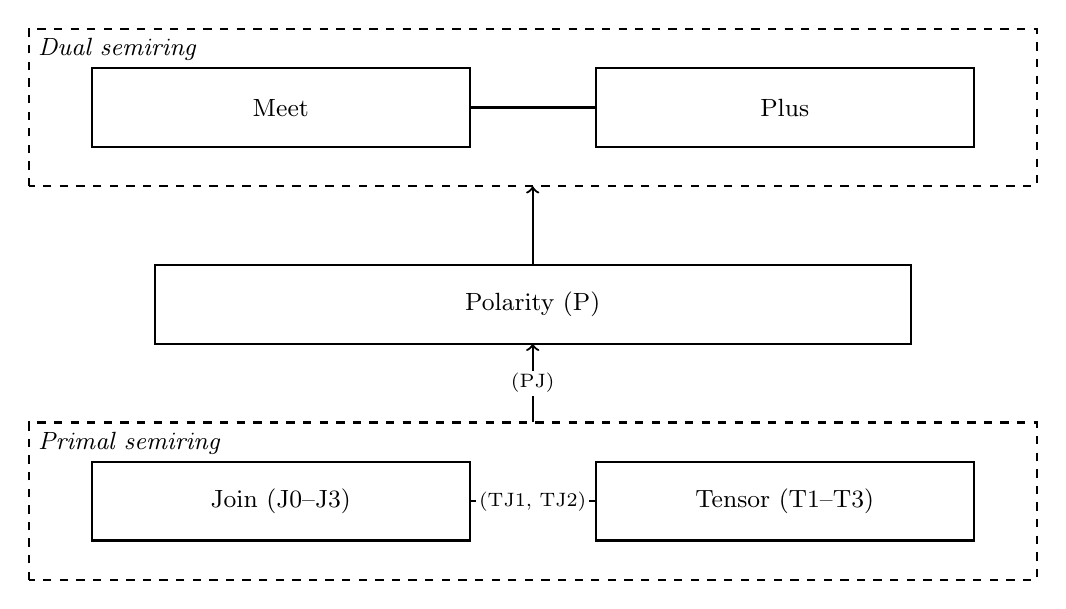
\begin{tikzpicture}[x=\xunit, y=\yunit, thick, font=\small]

% ===================================================================
% Integer grid. Each box given by bottom-left (BL) and top-right (TR).
% Outer boxes are 16 units wide; inner boxes are 6 units wide with a
% 2-unit gap, so BL/TR and all centers land on integers.
% Layout, bottom to top: Primal semiring / Polarity / Dual semiring.
% ===================================================================

% ---- Primal semiring: outer box (0,0) to (16,4) ----
\draw[dashed] (0,0) rectangle (16,4);
\node[anchor=north west, inner sep=3pt] at (0,4) {\itshape Primal semiring};

% Join: BL (1,1) TR (7,3), center (4,2)
\draw (1,1) rectangle (7,3);
\node[align=center] at (4,2) {Join (J0--J3)};

% Tensor: BL (9,1) TR (15,3), center (12,2)
\draw (9,1) rectangle (15,3);
\node[align=center] at (12,2) {Tensor (T1--T3)};

% intra-layer edge: Join -- Tensor, at mid-height y=2
\draw (7,2) -- (9,2);
\node[fill=white, inner sep=1pt] at (8,2) {\scriptsize (TJ1, TJ2)};

% ---- Polarity: BL (2,6) TR (14,8), center (8,7) ----
\draw (2,6) rectangle (14,8);
\node at (8,7) {Polarity $(\mathrm{P})$};

% ---- Dual semiring: outer box (0,10) to (16,14) ----
\draw[dashed] (0,10) rectangle (16,14);
\node[anchor=north west, inner sep=3pt] at (0,14) {\itshape Dual semiring};

% Meet: BL (1,11) TR (7,13), center (4,12)
\draw (1,11) rectangle (7,13);
\node at (4,12) {Meet};

% Plus: BL (9,11) TR (15,13), center (12,12)
\draw (9,11) rectangle (15,13);
\node at (12,12) {Plus};

% intra-layer edge: Meet -- Plus, at mid-height y=12
\draw (7,12) -- (9,12);
% \node[fill=white, inner sep=1pt] at (8,12) {\scriptsize (RS3)};

% ---- vertical links: outer box to outer box, both centered at x=8 ----
\draw[->] (8,4) -- (8,6) node[midway, fill=white, inner sep=1pt] {\scriptsize (PJ)};
% \draw[->] (8,4) -- (8,6);
\draw[->] (8,8) -- (8,10);

\end{tikzpicture}
\caption{The axiomatic modules of a Polar Semiring. The primal semiring
$(X,\vee,\otimes,e_\vee,e_\otimes)$ and its dual $(X,\wedge,\oplus,e_\wedge,e_\oplus)$
are related through the polarity, which supplies axioms (P) and (PJ).}
\label{fig:architecture}
\end{figure}


\subsection{Algebraic layer}\label{subsec:algebraic}

The algebraic layer consists of two independent modules and their
interaction:
\begin{enumerate}
  \item the \emph{join module} $(X,\vee,\ev)$, an idempotent commutative
  monoid by \eqref{ax:J0}--\eqref{ax:J3};
  \item the \emph{tensor module} $(X,\otimes,\eo)$, a commutative monoid by
  \eqref{ax:T1}--\eqref{ax:T3};
  \item the interaction axioms \eqref{ax:TJ1}--\eqref{ax:TJ2}, which make
  $(X,\vee,\otimes,\ev,\eo)$ an idempotent commutative semiring
  \citep{Golan1999}.
\end{enumerate}
The join module already carries order-theoretic information: by
\eqref{ax:J0}--\eqref{ax:J2}, the relation $\leq$ of \eqref{eq:orders} is a
partial order (reflexivity is \eqref{ax:J0}, antisymmetry follows from
\eqref{ax:J2}, transitivity from \eqref{ax:J1}), with least element $\ev$ by
\eqref{ax:J3}, and $a \vee b$ is the least upper bound of $a$ and $b$. The
interaction axioms give monotonicity of the tensor:

\begin{lemma}\label{lem:tensor-monotone}
In any Polar Semiring, $a \leq b$ implies $a \otimes c \leq b \otimes c$.
\end{lemma}

\begin{proof}
If $a \vee b = b$, then by \eqref{ax:TJ1} and \eqref{ax:T2},
$(a \otimes c) \vee (b \otimes c) = (a \vee b) \otimes c = b \otimes c$.
\end{proof}

Nothing in this layer mentions ${}^{*}$: it is ordinary semiring theory.

\subsection{Reflection layer}\label{subsec:reflection}

We now add the involution axiom \eqref{ax:P} and nothing else, and show
that it \emph{reflects} each module of the algebraic layer into a dual
module, with all duality laws obtained for free. We first fix terminology.
Following the historical order of the notions---involutions belong to pure
algebra, polarities to order theory \citep{Birkhoff1940}---we call a
structure \emph{involutive} when it satisfies only
$\dstar{(\dstar{a})} = a$, and reserve the adjective \emph{polar} for
structures in which the involution is additionally compatible with the
induced order via \eqref{ax:PJ}. Thus an \emph{involutive commutative
monoid} is a commutative monoid equipped with an involution; no order is
involved, and indeed at this level no order need exist.

\begin{proposition}[Duality laws]\label{prop:duality}
Let $(X,\vee,\ev)$ and $(X,\otimes,\eo)$ be commutative monoids and let
${}^{*}$ satisfy \eqref{ax:P}. With the derived operations
\eqref{eq:derived-ops}, the following hold for all $a,b \in X$:
\begin{align}
  \dstar{(a \wedge b)} &= \dstar{a} \vee \dstar{b},
    \label{eq:RD1}\\
  \dstar{(a \oplus b)} &= \dstar{a} \otimes \dstar{b},
    \label{eq:RD2}\\
  \dstar{(a \vee b)} &= \dstar{a} \wedge \dstar{b},
    \label{eq:RD3}\\
  \dstar{(a \otimes b)} &= \dstar{a} \oplus \dstar{b},
    \label{eq:RD4}\\
  \dstar{\ev} = \ew,\quad \dstar{\ew} = \ev,&\quad
  \dstar{\eo} = \ep,\quad \dstar{\ep} = \eo.
    \label{eq:RD5}
\end{align}
\end{proposition}

\begin{proof}
For \eqref{eq:RD1}, apply \eqref{ax:P} to the definition:
$\dstar{(a \wedge b)}
 = \dstar{(\dstar{(\dstar{a} \vee \dstar{b})})}
 = \dstar{a} \vee \dstar{b}$.
For \eqref{eq:RD3}, compute
$\dstar{a} \wedge \dstar{b}
 = \dstar{(\dstar{(\dstar{a})} \vee \dstar{(\dstar{b})})}
 = \dstar{(a \vee b)}$ by \eqref{ax:P}. Equations \eqref{eq:RD2} and
\eqref{eq:RD4} are identical computations with $\otimes,\oplus$ in place of
$\vee,\wedge$. In \eqref{eq:RD5}, the first and third equations are the
definitions in \eqref{eq:derived-ops}, and the other two follow by
\eqref{ax:P}.
\end{proof}

\begin{proposition}[Reflected modules]\label{prop:reflected-modules}
Under the hypotheses of \Cref{prop:duality}:
\begin{enumerate}
  \item $(X,\wedge,\ew)$ is a commutative monoid, the \emph{meet module};
  \item $(X,\oplus,\ep)$ is a commutative monoid, the \emph{plus module};
  \item if moreover \eqref{ax:J0} holds, then $\wedge$ is idempotent.
\end{enumerate}
\end{proposition}

\begin{proof}
Commutativity of $\wedge$ is immediate from \eqref{ax:J2}. For
associativity, using \eqref{eq:RD1},
\[
  (a \wedge b) \wedge c
  = \dstar{\bigl(\dstar{(a \wedge b)} \vee \dstar{c}\bigr)}
  = \dstar{\bigl((\dstar{a} \vee \dstar{b}) \vee \dstar{c}\bigr)},
\]
and \eqref{ax:J1} lets the inner join reassociate; reversing the steps gives
$a \wedge (b \wedge c)$. For the unit,
$a \wedge \ew
 = \dstar{(\dstar{a} \vee \dstar{\ew})}
 = \dstar{(\dstar{a} \vee \ev)}
 = \dstar{(\dstar{a})} = a$
by \eqref{eq:RD5}, \eqref{ax:J3}, and \eqref{ax:P}. Item (2) is the same
argument in the tensor module, using \eqref{ax:T1}--\eqref{ax:T3}. For (3),
$a \wedge a = \dstar{(\dstar{a} \vee \dstar{a})} = \dstar{(\dstar{a})} = a$
by \eqref{ax:J0} and \eqref{ax:P}.
\end{proof}

Two comments are in order. First, everything above is a consequence of the
involution equation alone; the reflection layer is \emph{axiomatically
free}. Second, at this stage the two relations $\leq$ and $\leqm$ of
\eqref{eq:orders} are both available, but nothing yet guarantees that they
coincide, nor that $\wedge$ computes greatest lower bounds with respect to
$\leq$. That is precisely the task of the third layer.

\subsection{Integration layer}\label{subsec:integration}

The final axiom \eqref{ax:PJ} is the first, and only, axiom relating the
polarity to the join module, and it is not derivable from the previous
layers (\Cref{thm:independence}). Its effect is to integrate the reflected
order with the original one.

\begin{proposition}[Order compatibility]\label{prop:order-compat}
In the presence of the other ten axioms, the following are equivalent:
\begin{enumerate}
  \item \eqref{ax:PJ}: $a \vee b = b \iff \dstar{b} \vee \dstar{a} = \dstar{a}$;
  \item $a \vee b = b \iff b \wedge a = a$;
  \item $a \leq b \iff \dstar{b} \leqm \dstar{a}$;
  \item the absorption laws:
  $a \wedge (a \vee b) = a$ and $a \vee (a \wedge b) = a$.
\end{enumerate}
\end{proposition}

\begin{proof}
(1)$\Leftrightarrow$(2): by \eqref{eq:derived-ops} and \eqref{ax:P},
$b \wedge a = a$ holds if and only if
$\dstar{(\dstar{b} \vee \dstar{a})} = a$, if and only if
$\dstar{b} \vee \dstar{a} = \dstar{a}$; so (2) is a literal restatement of
(1).

(1)$\Leftrightarrow$(3): unfolding \eqref{eq:orders},
$\dstar{b} \leqm \dstar{a}$ means $\dstar{b} \wedge \dstar{a} = \dstar{b}$,
that is, $\dstar{(b \vee a)} = \dstar{b}$ by \eqref{eq:RD3}, that is,
$b \vee a = a$ by injectivity of ${}^{*}$; renaming variables shows (3) to
be a restatement of (1) as well.

(2)$\Rightarrow$(4): since $a \leq a \vee b$ by
\eqref{ax:J0}--\eqref{ax:J1}, item (2) yields
$(a \vee b) \wedge a = a$, which is the first absorption law by
commutativity of $\wedge$. For the second, (2) applied in the direction
``$b \wedge a = a \Rightarrow a \vee b = b$'' with the pair
$(a \wedge b, a)$: indeed $a \wedge (a \wedge b) = a \wedge b$ by
idempotence and associativity of $\wedge$
(\Cref{prop:reflected-modules}), so $(a \wedge b) \vee a = a$, which is
the second absorption law.

(4)$\Rightarrow$(2): if $a \vee b = b$, then
$a \wedge b = a \wedge (a \vee b) = a$, so $b \wedge a = a$. Conversely, if
$b \wedge a = a$, then $a \vee b = (b \wedge a) \vee b = b$ by the second
absorption law and commutativity.
\end{proof}

\begin{proposition}[Order structure]\label{prop:order-structure}
In any Polar Semiring:
\begin{enumerate}
  \item $\leq$ is a partial order and $\leq \;=\; \leqm$;
  \item $\ev \leq a \leq \ew$ for all $a$;
  \item $a \leq b$ implies $a \wedge c \leq b \wedge c$ and
        $a \oplus c \leq b \oplus c$;
  \item $a \vee b$ is the least upper bound and $a \wedge b$ the greatest
        lower bound of $\{a,b\}$ with respect to $\leq$; consequently
        $(X,\vee,\wedge)$ is a (possibly non-distributive) lattice.
\end{enumerate}
\end{proposition}

\begin{proof}
(1) That $\leq$ is a partial order was noted in \Cref{subsec:algebraic}.
By \Cref{prop:order-compat}(2), $a \leq b$ if and only if $a \wedge b = a$,
which is $a \leqm b$; hence the two orders coincide.

(2) $\ev \leq a$ is \eqref{ax:J3} with \eqref{ax:J2}. For $a \leq \ew$: by
\eqref{ax:PJ} this is equivalent to
$\dstar{\ew} \vee \dstar{a} = \dstar{a}$, that is,
$\ev \vee \dstar{a} = \dstar{a}$, which holds by \eqref{ax:J3}.

(3) Suppose $a \leq b$, so $a \wedge b = a$ by
\Cref{prop:order-compat}(2). Then
$(a \wedge c) \wedge (b \wedge c) = (a \wedge b) \wedge (c \wedge c)
 = a \wedge c$
by \Cref{prop:reflected-modules}, whence $a \wedge c \leqm b \wedge c$, and
we conclude by (1). For $\oplus$: from $a \leq b$,
\eqref{ax:PJ} gives $\dstar{b} \leq \dstar{a}$, then
\Cref{lem:tensor-monotone} gives
$\dstar{b} \otimes \dstar{c} \leq \dstar{a} \otimes \dstar{c}$, and applying
\eqref{ax:PJ} once more together with \eqref{eq:RD2} yields
$a \oplus c \leq b \oplus c$.

(4) The least-upper-bound property of $\vee$ is standard in idempotent
commutative monoids: $a,b \leq a \vee b$, and if $a,b \leq c$ then
$(a \vee b) \vee c = c$. For $\wedge$, dualize: by \eqref{ax:PJ} and
\eqref{eq:RD3}, lower bounds of $\{a,b\}$ correspond under ${}^{*}$ to upper
bounds of $\{\dstar{a},\dstar{b}\}$, and the correspondence sends
$a \wedge b$ to $\dstar{a} \vee \dstar{b}$; the greatest-lower-bound
property follows. The absorption laws of \Cref{prop:order-compat}(4) then
exhibit $(X,\vee,\wedge)$ as a lattice, bounded by (2). Distributivity of
$\vee$ over $\wedge$ is not asserted and indeed fails in general.
\noteAI{If you want a concrete non-distributive example here, add the
diamond $M_3$ with a suitable involution and check
\eqref{ax:TJ1}--\eqref{ax:TJ2} for a chosen tensor; otherwise the claim
``fails in general'' should be softened or given a citation.}
\end{proof}

The structure obtained from the join module together with \eqref{ax:P} and
\eqref{ax:PJ} alone---a bounded, possibly non-distributive lattice with an
antitone involution satisfying the De Morgan laws---is what we call a
\emph{Polar Lattice}; it coincides with the classical notion of a bounded
i-lattice \citep{Kalman1958}. We return to this identification in the
orientation table of \Cref{sec:positioning}.

\subsection{The Fundamental Structure Theorem}\label{subsec:fundamental}

Assembling the three layers yields the main theorem of this section.

\begin{theorem}[Fundamental Structure Theorem]\label{thm:fundamental}
Let $(X,\vee,\otimes,{}^{*},\ev,\eo)$ be a Polar Semiring. Then:
\begin{enumerate}
  \item the \emph{dual structure} $(X,\wedge,\oplus,{}^{*},\ew,\ep)$ is
  again a Polar Semiring;
  \item the polarity ${}^{*}\colon X \to X$ is an isomorphism from
  $(X,\vee,\otimes,{}^{*},\ev,\eo)$ onto its dual;
  \item the join order of the original structure and the meet order induced
  by the dual structure coincide, in the sense that
  $\leq \;=\; \leqm$.
\end{enumerate}
\end{theorem}

\begin{proof}
(1) We verify the eleven axioms for
$(X,\wedge,\oplus,{}^{*},\ew,\ep)$. Axioms J0--J3 for $\wedge$ and T1--T3
for $\oplus$ are \Cref{prop:reflected-modules}. Axiom P is unchanged. For
the dual of \eqref{ax:TJ1}, using \eqref{eq:RD1}--\eqref{eq:RD4} and
\eqref{ax:TJ1} in the original structure,
\[
  a \oplus (b \wedge c)
  = \dstar{\bigl(\dstar{a} \otimes (\dstar{b} \vee \dstar{c})\bigr)}
  = \dstar{\bigl((\dstar{a} \otimes \dstar{b}) \vee
                 (\dstar{a} \otimes \dstar{c})\bigr)}
  = (a \oplus b) \wedge (a \oplus c).
\]
For the dual of \eqref{ax:TJ2},
$a \oplus \ew
 = \dstar{(\dstar{a} \otimes \ev)}
 = \dstar{\ev} = \ew$
by \eqref{eq:RD5} and \eqref{ax:TJ2}. Finally, the dual of \eqref{ax:PJ}
asserts $a \wedge b = b \iff \dstar{b} \wedge \dstar{a} = \dstar{a}$; by
\Cref{prop:order-compat}(2) and \Cref{prop:order-structure}(1), both sides
translate to statements about $\leq$, namely $b \leq a$ on the left and
$\dstar{a} \leq \dstar{b}$ on the right, and these are equivalent by
\eqref{ax:PJ}.

(2) The map ${}^{*}$ is a bijection by \eqref{ax:P}, and
\eqref{eq:RD3}--\eqref{eq:RD5} say exactly that it sends $\vee$ to
$\wedge$, $\otimes$ to $\oplus$, $\ev$ to $\ew$, and $\eo$ to $\ep$; it
commutes with itself trivially. Hence it is an isomorphism onto the dual
structure.

(3) This is \Cref{prop:order-structure}(1).
\end{proof}

\begin{remark}
The theorem justifies the architectural reading of the axiom system: the
algebraic layer supplies the raw modules, the reflection layer produces the
dual modules for free from \eqref{ax:P}, and the single integration axiom
\eqref{ax:PJ} welds the two orders together, at which point the duality
becomes a self-duality of the whole structure. In particular, applying the
construction twice returns the original Polar Semiring, since
$\dstar{(\dstar{a})} = a$.
\end{remark}
